\section{Preparació de variables}

\subsection{Normalització i escalat de variables}
En les variables numèriques, s'ha considerat l'ús de dues tècniques diferents per a l'escalat de dades: \textit{Standard Scaler} i \textit{MinMax Scaler}. El \textit{Standard Scaler} transforma les dades de manera que tinguin una mitjana de zero i una desviació estàndard d'una, mentre que el \textit{MinMax Scaler} redimensiona les dades en un rang entre 0 i 1.

Tenint en compte la nostra base de dades i l'ús que farem de les varianbles numèriques (princpalment per trobar distàncies entre mostres, etc.), s'ha decidit que, en general, el \textit{MinMax Scaler} és més útil o té més sentit per a la nostra aplicació. Aquesta decisió es basa en la manera en què el \textit{MinMax Scaler} preserva la relació entre les variables originals (mantenint les mateixes distàncies relatives), sent particularment beneficiós quan les característiques estan en diferents escales.

La normalització o l'escalat pot millorar significativament el rendiment dels nostres models (KNN, arbre de decisió i SVM), ja que es basen en les distàncies entre les punts o en la definició de marges entre les classes. Per tant, si s'ha de realitzar algun escalat es farà \textit{MinMax}. Arà bé, més endavant es valorarà per cada model si és millor realitzar ecalat o no.

Cal mencionar que escalat de dades es realitza sempre per separat en train i test, per tal de no tenir fuga de dades d'un conjunt a l'altre. A més, es fa abans d'imputar els valors faltants, ja que així els models d'imputació es poden beneficiar també dels avantatges de l'escalat de dades.

\subsection{Anàlisi de correlacions entre variables numèriques}
Per poder analitzar la correlació entre variables numèriques del dataset d'entrenament, s'ha fet una matriu de correlacions. No obstant, com ja s'ha mencionat, és possible que no s'utilitzi exactament la mateixa base de dades per entrenar tots els models. Per exemple, pot ser que en algun model es faci escalat de dades i en algun altre no, en algun s'eliminin outliers i en un altre no, etc..

Donada la gran quantitat de datasets d'entrenament que podem tenir en funció de les modificacions que hi fem, per realitzar la matriu de correlacions s'ha decidir fixar una llavor (\textit{seed}) per poder replicar els experiments i s'ha tingut en compte el dataset d'entrenament reultant a l'aplicar els següents canvis:
\begin{itemize}
	\item Llavor (random\_state) establerta arbitràriament al valor 42 en tots els processos que tinguin aleatorietat.
	\item Eliminació d'oultliers (amb factor multiplicatiu del IQR de 3).
	\item Sense eliminar les files amb 9 missings.
	\item Sense codificació de variables categòriques (això no hauria d'influir en les correlacions de variables numèriques, però s'especifica per si de cas).
	\item Escalat de variables numèriques mitjançant \textit{MinMax}.
	\item Missings imputats mitjançant els imputadors amb millors resultats amb la llavor escollida (mitjançant la funció \texttt{find\_best\_imputer()}) i determinats mitjançant la mètrica de $R^2$ (per variables numèriques) i \textit{f1-score-weighted} (per variables categòriques). Amb tot això, per a variables numèriques ha resultat ser millor l'IterativeImputer (amb Lineal Regression com a estimador), mentre que per a variables categòriques ha sigut el RandomForestClassifier amb el criteri gini.
	\item Sense realitzar cap mètode de balanceig de dades (explicats més endavant).
\end{itemize}

Tenint en compte totes aquestes consideracions, la matriu de correlacions entre variables numèriques resultant és la que es pot veure en la figura \ref{fig:num-corr}.

\begin{figure}[H]
	\centering
	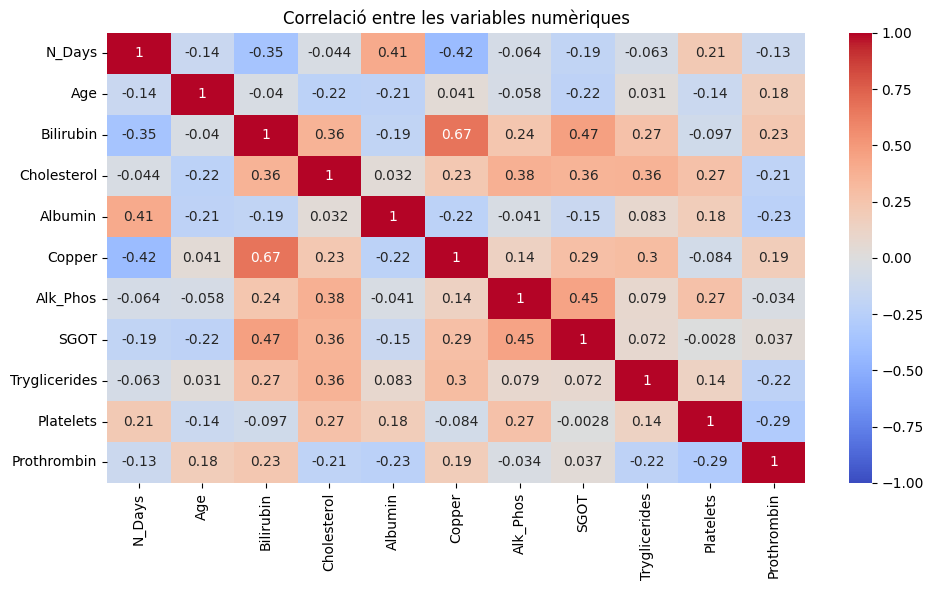
\includegraphics[width=0.9\linewidth]{img/num-corr.png}
	\caption{Matriu de correlacions entre totes les parelles de variables numèriques.}
	\label{fig:num-corr}
\end{figure}

Cal mencionar que la matriu de correlacions que es pot observar a la figura \ref{fig:num-corr} ens diu el coeficient de correlació per cada parella de variables, basant-se només en relacions lineals entre elles. Per tant, és possible que algunes de les variables numèriques tinguin clares relacions no lineals, però això no es pot apreciar en aquesta matriu.

La correlació entre \textit{Bilirubin} i \textit{Copper} és de 0,67, la qual cosa indica una forta correlació positiva. Això significa que a mesura que el valor de \textit{Bilirubin} augmenta, el valor de \textit{Copper} també tendeix a augmentar. 

\textit{Bilirubin} i \textit{SGOT} tenen una correlació positiva de 0,47, també bastant forta; i \textit{SGOT} i \textit{Alk\_Phos} de 0,45.

\textit{Copper} i \textit{N\_Days} destaquen pel que fa a les correlacions negatives, amb un coeficient de $-0,42$.

Finalment, la variable \textit{Cholesterol} té fins a 3 coeficients de correlació amb valors de 0,38, 0,36 i 0,36 amb les variables \textit{Alk\_Phos}, \textit{SGOT} i \textit{Tryglicerides}, respectivament.

Una vegada analitzades les correlacions més fortes, podem veure que les variables \textit{Bilirubin}, \textit{Copper}, \textit{SGOT} i \textit{Alk\_Phos} són les que es troben en més correlacions més fortes entre variables.

És important destacar que una correlació no implica causalitat. Això significa que, encara que dues variables estiguin correlacionades, no es pot assegurar que el valor d'una sigui causant del valor de l'altre. Per tant, no podem dir que el valor d'aquestes tres variables depengui dels altres, però en el nostre dataset d'entrenament es dona la casualitat (o potser causalitat) de que hi ha una alta correlació entre aquestes variables i altres variables del dataset.

Sabent tot això, si s'hagués d'eliminar alguna variable, les millors opcions per variables numèriques serien alguna de les 4 que hem mencionat, ja que part de la informació que aporten ja està explicada per altres variables. No obstant, s'ha considerat que, per la tasca de predicció de la variable objectiu i tenint en compte les dimensions del dataset, no cal eliminar cap variable numèrica per motiu de la seva correlació amb altres variables numèriques.

\subsection{Anàlisi de variables categòriques i variable objectiu}
Com que l'objectiu d'aquest projecte és acabar predint el valor de la variable \textit{Status}, és molt important veure com influeix el valor de la variable objectiu en cada variable categòrica.

Abans de res, cal mencionar que aquestes relacions han estat estudiades amb la mateixa base de dades d'entrenament que en l'apartat anterior. És a dir, aplicant exactament les mateixes modificacions al dataset inicial per tal de tenir el mateix conjunt de train. En funció del model que s'utilitzi posteriorment, aquest conjunt d'entrenament pot variar lleugerament.

En les figures \ref{fig:cat-target-1} i \ref{fig:cat-target-2} es poden veure aquestes relacions. Si entre els les diferents classes de la variable categòrica hi ha una distribució similar dels valors de la variable \textit{Status}, això ens indica que aquella variable categòrica no té gaire influència en la variable objectiu. Aquest és el cas de variables com \textit{Drug}.

Per altra banda, es pot veure que no hi ha cap variable amb una gran influència cap a la variable objectiu. A més, es destaca el desbalanceig de la variable objectiu, que tractarem a continuació. 

Amb tot el que s'ha vist, podem dir que si fos necessari eliminar una variable categòrica de l'entrenament, es podria eliminar la variable \textit{Drug}, ja que sembla ser la que menys influeix en la variable objectiu. No obstant, s'ha considerat que no és necessari eliminar-la degut a les característiques del nostre dataset.

És interessant observar que, si ens parem a pensar en la conclusió d'aquest anàlisi, s'ha mencionat que la variable \textit{Drug} (que originalment tenia valors `D-penicillamine' i `Placebo', i al preprocessing inicial s'han reemplaçat per 1 i 0, respectivament) no té pràcticament influència en la variable \textit{Status} (que indica si un pacient ha sobreviscut o no a la malaltia). Per tant, això ens està indicant que el tractament que es va utilitzar per realitzar aquest estudi sobre la cirrosis hepàtica no era efectiu. És a dir, els pacients que se'ls proporcionava el tractament (\textit{Drug} = `D-penicillamine', ara modificat a \textit{Drug} = 1) tenien les mateixes possibilitats de morir/sobreviure que els pacients que se'ls proporcionava un simple placebo.

\begin{figure}[H]
\centering
\begin{subfigure}[b]{0.5\textwidth}
    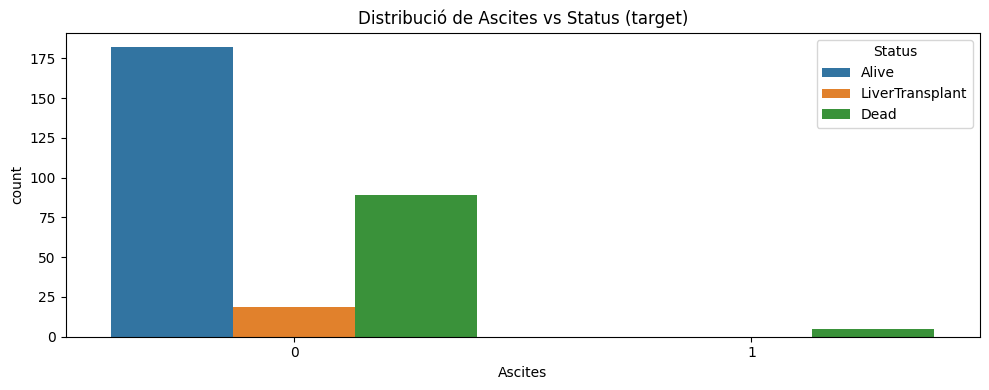
\includegraphics[width=\textwidth]{img/corr_Ascites_vs_status.png}
    \caption{Ascites vs status}
    \label{fig:ascites_vs_status}
\end{subfigure}%
\begin{subfigure}[b]{0.5\textwidth}
    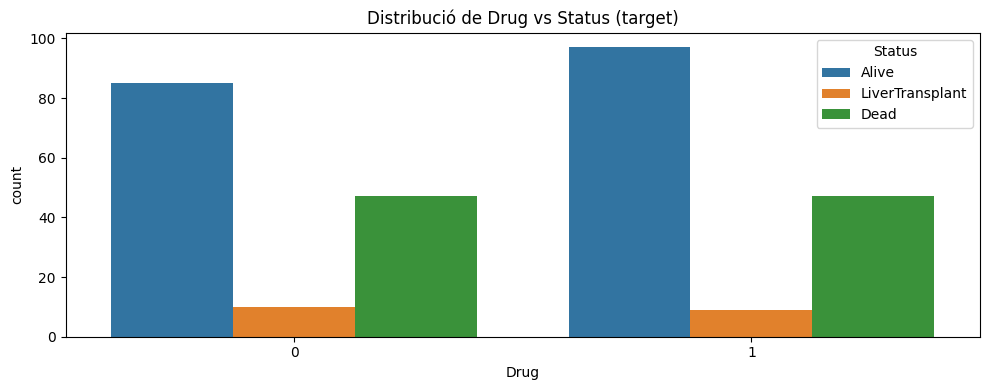
\includegraphics[width=\textwidth]{img/corr_Drug_vs_status.png}
    \caption{Drug vs status}
    \label{fig:drug_vs_status}
\end{subfigure}
\begin{subfigure}[b]{0.5\textwidth}
    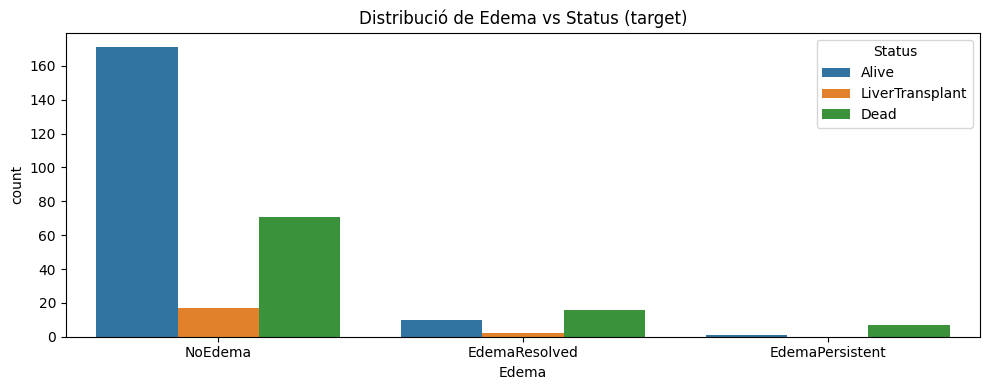
\includegraphics[width=\textwidth]{img/corr_Edema_vs_status.png}
    \caption{Edema vs status}
    \label{fig:edema_vs_status}
\end{subfigure}%
\begin{subfigure}[b]{0.5\textwidth}
    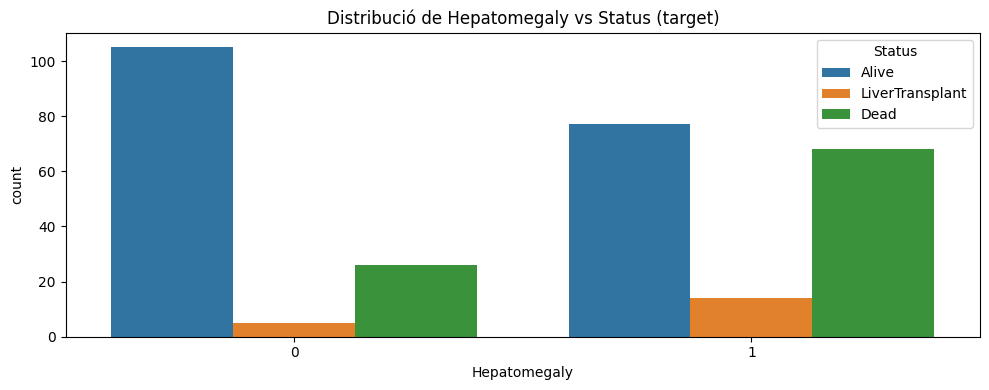
\includegraphics[width=\textwidth]{img/corr_Hepatomegaly_vs_status.png}
    \caption{Hepatomegaly vs status}
    \label{fig:hepatomegaly_vs_status}
\end{subfigure}
\caption{Relació entre les variables categòriques i la variable objectiu (\textit{Status})}
\label{fig:cat-target-1}
\end{figure}

\begin{figure}[H]
\centering
\begin{subfigure}[b]{0.5\textwidth}
    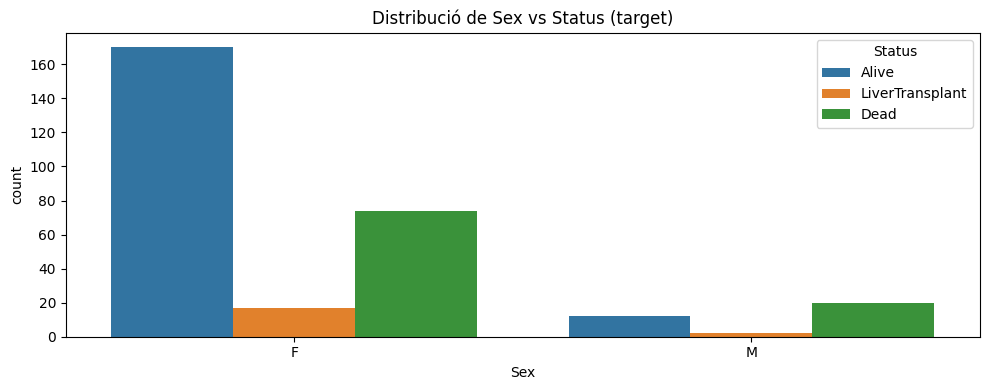
\includegraphics[width=\textwidth]{img/corr_Sex_vs_status.png}
    \caption{Sex vs status}
    \label{fig:sex_vs_status}
\end{subfigure}%
\begin{subfigure}[b]{0.5\textwidth}
    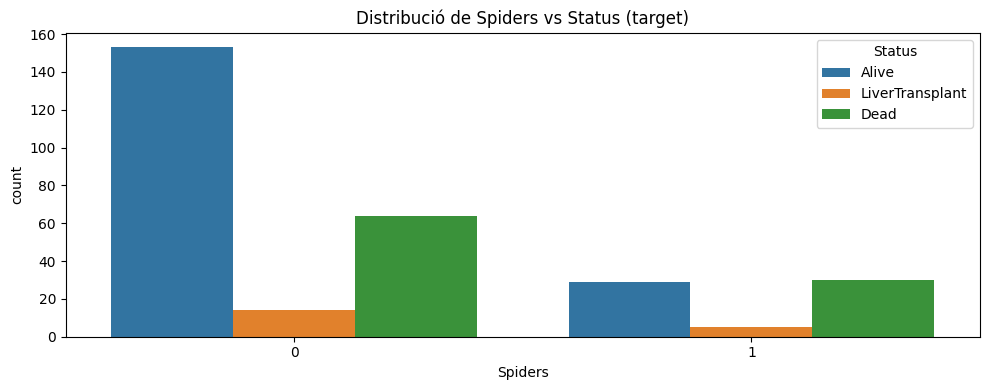
\includegraphics[width=\textwidth]{img/corr_Spiders_vs_status.png}
    \caption{Spiders vs status}
    \label{fig:spiders_vs_status}
\end{subfigure}
\begin{subfigure}[b]{0.5\textwidth}
    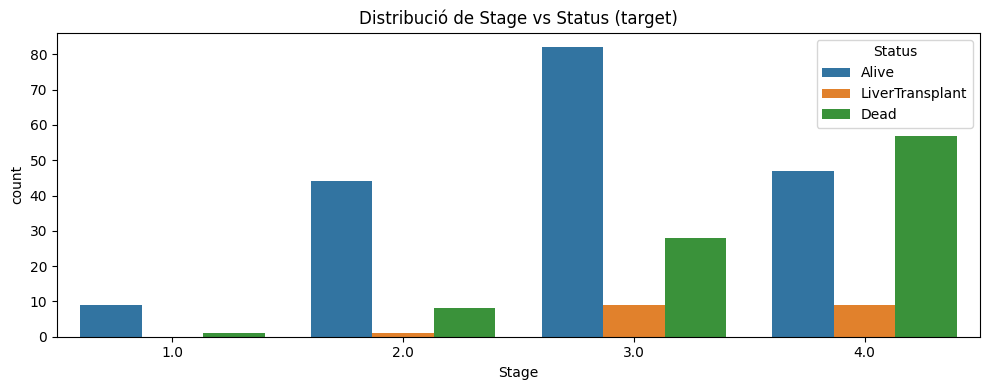
\includegraphics[width=\textwidth]{img/corr_Stage_vs_status.png}
    \caption{Stage vs status}
    \label{fig:stage_vs_status}
\end{subfigure}%
\begin{subfigure}[b]{0.5\textwidth}
    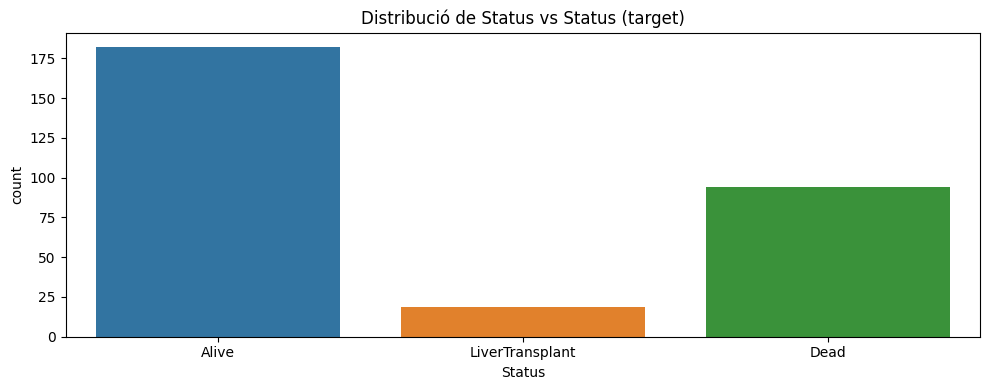
\includegraphics[width=\textwidth]{img/corr_Status_vs_status.png}
    \caption{Status vs status}
    \label{fig:status_vs_status}
\end{subfigure}
\caption{Relació entre les variables categòriques i la variable objectiu (\textit{Status})}
\label{fig:cat-target-2}
\end{figure}

\subsection{Balanceig de classes de la variable objectiu}
Com ja hem vist en la figura \ref{fig:status_vs_status}, la variable objectiu (\textit{Status}) està clarament desbalancejada. Hi ha moltes mostres amb valor `Alive', unes quantes amb valor `Dead' i molt poques amb valor `LiverTransplant'.

Això pot causar que els nostres models es dediquin a predir la classe majoritària i tinguin molt mal rendiment predient valors de la classe minoritària. Per poder solucionar-ho, s'han implementat diversos mètodes de balanceig de dades en la funció \texttt{balance\_target\_classes()} per aplicar al conjunt d'entrenament. En concret, s'ha implementat Oversampling, Undersampling, SMOTE i SMOTEENN.

Degut a la poca quantiat de dades del nostre dataset, ja podem saber que no té cap mena de sentit intentar aplicar Undersample, ja que ens quedaríem amb molt poques dades en el conjunt d'entrenament.

El mètode de Oversampling pot ser útil degut a la seva senzillesa. Simplement replica mostres del datset fins que les classes estan equilibrades. No obstant, s'ha d'anar amb compte amb aquest mètode perquè pot provocar overfitting.

El mètodes de SMOTE consisteix en generar mostres sintètiques basant-se en combinacions lineals dels veïns més propers. Aquest mètode és computacionalment més car, però redueix el risc de sobreajustament (overfitting) en comparació al Oversample.

Finalment, el mètode SMOTEENN es basa en un SMOTE, però posteriorment elimina aquelles mostres que considera de pitjor qualitat. Aconsegueix un menor balanceig de classes però assegura una millor qualitat de les mostres generades sintèticament.

Tots aquests mètodes es provaran més endavant per cada model i es determinarà quin és el que proporciona millors resultats per a cada un. Cal mencionar que tant SMOTE com SMOTEENN requereixen que les dades hagin estat codificades, ja que no poden tractar valors que no siguin numèrics. Així doncs, quan el dataset no ha estat codificat, no es podrà aplicar cap d'aquests dos mètodes.

\subsection{Eliminació de variables}
Pel que fa a la eliminació de possibles variables, ja s'ha mencionat en apartats anteriors que no s'ha considerat necessari en aquest projecte. El dataset té una mida relativament petita i no hi ha variables extremadament redundants o sorolloses. Per tant, eliminar variables no és necessari.

En cas que es volgués eliminar alguna variable numèrica, ja s'ha mencionat que les millors opcions serien \textit{Bilirubin}, \textit{Copper}, \textit{SGOT} o \textit{Alk\_Phos}. Per altra banda, en les variables categòriques s'optaria per eliminar \textit{Drug}.

\subsection{Estudi de dimensionalitat (ACP)}
En aquest apartat s'ha realitzat un estudi sobre la dimensionalitat de la base de dades d'entrenament mitjançant l'Anàlisi de Components Principals (ACP o PCA).

En la figura \ref{fig:acp-cum-var} es pot veure el percentatge de variància explicada en funció del nombre de components principals. Es pot veure que amb els 7 primers components principals ja s'explica un 80\% de la variància. Per tant, en cas que es desitgés fer una reducció de la dimensionalitat, amb tan sols 7 components principals (en comptes de les 11 variables numèriques que hi ha ara) es podria explicar un 80\% de la variància, que generalment es considera suficient per no perdre informació rellevant i fins i tot eliminar soroll o redundància.

\begin{figure}[H]
	\centering
    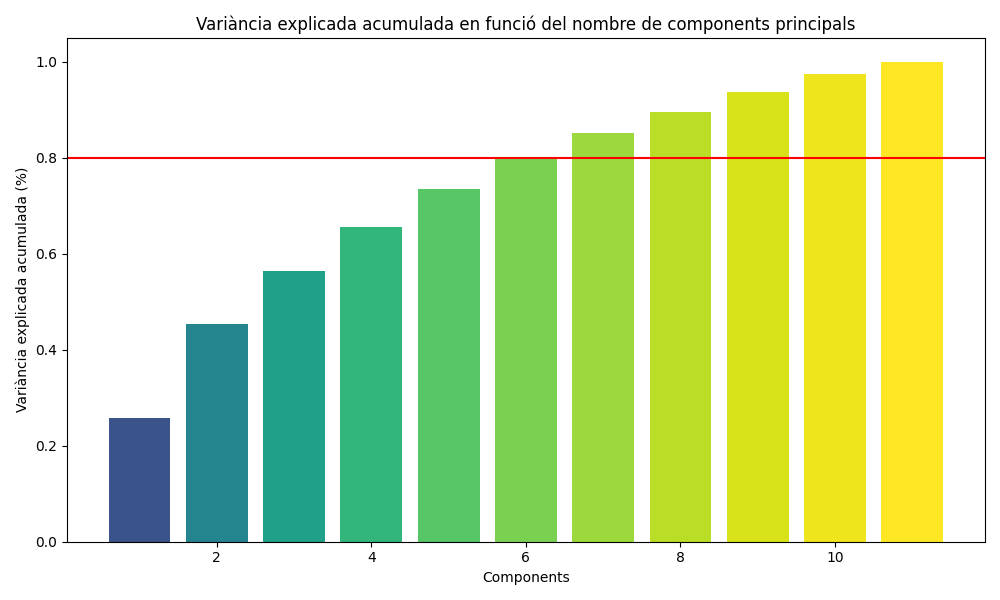
\includegraphics[width=0.9\textwidth]{img/acp_cum_explained_variance.png}
    \caption{Percentatge de variància explicada en funció del nombre de components principals.}
    \label{fig:acp-cum-var}
\end{figure}

En la figura \ref{fig:acp-num-proj} es poden veure les projeccions de les variables numèriques en els dos primers eixos principals. El primer eix principal explica un 25,77\% de la variància i el segon un 19,64\% de la variància, de manera que tenim aproximadament un 45\% de la variància explicada. Amb això, les conclusions que extraiem d'aquí s'han de tractar amb molt de compte, ja que no seran conclusions extretes de tota la informació del dataset, sinó d'aproximadament la meitat. Es pot apreciar, com ja hem mencionat en l'anàlisi de correlacions entre variables numèriques, que les variables \textit{Bilirubin}, \textit{Copper} i \textit{SGOT} estan bastant relacionades, i en aquest cas veiem que es projecten bastant sobre el primer eix principal.

Per tant, el primer eix principal es caracteritza princpalment per els valors positius de \textit{Bilirubin}, \textit{Copper}, \textit{SGOT} i lleugerament \textit{Cholesterol}; i els valors negatius (relació inversa) lleugerament amb \textit{N\_Days}.

Pel que fa al segon eix principal, veiem que hi té projectades positivament \textit{Age} i \textit{Prothrombin}; i negativament sobretot \textit{Platelets}, però també lleugerament \textit{Cholesterol} i \textit{Albumin}. Amb la informació del segon eix, es podria dir que el valor de l'edat té una relació inversa amb el de \textit{Platelets}; és a dir, la gent més gran tendeix a tenir un valor de \textit{Platelets} més petit.

Resumint, es podria dir que el primer eix principal conté sobretot característiques sobre les dades mesurades del pacient, mentre que el segon component ve determinat especialment per l'edat i les plaquetes (platelets) del pacient.

\begin{figure}[H]
	\centering
    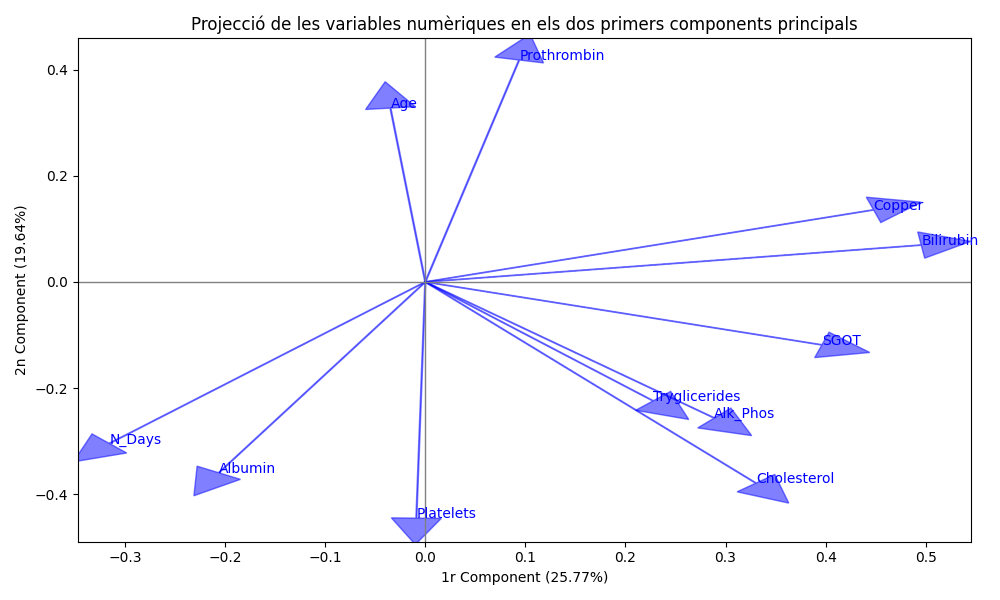
\includegraphics[width=0.9\textwidth]{img/acp_num_vars_projections.png}
    \caption{Projecció de les variables numèriques en els dos primers components principals.}
    \label{fig:acp-num-proj}
\end{figure}

Finalment, en la figura \ref{fig:acp-cat-proj} es pot veure la projecció dels centroides de les classes de les variables categòriques en els dos primers eixos principals. S'hi poden veure les classes de la variable target (\textit{Status}) clarament diferenciades. A més, hi ha curiositats com que el sexe masculí (M) es troba més aprop de `Dead' que el femení (F), indicant-nos que els homes tendeixen més a morir (\textit{Status} = `Dead') que les dones. També podem veure com el fet de tenir \textit{Spiders} o tenir \textit{Hepatomegaly} ``apropa'' al pacient cap a `Dead' (és a dir, en mitjana, és més probable que mori). Finalment, es pot mencionar la clara tendència de \textit{Stage} a apropar-se a `Dead' a mesura que augmenta el seu valor (com és lògic, en etapes més avançades de la malaltia és menys probable sobreviure).

\begin{figure}[H]
	\centering
    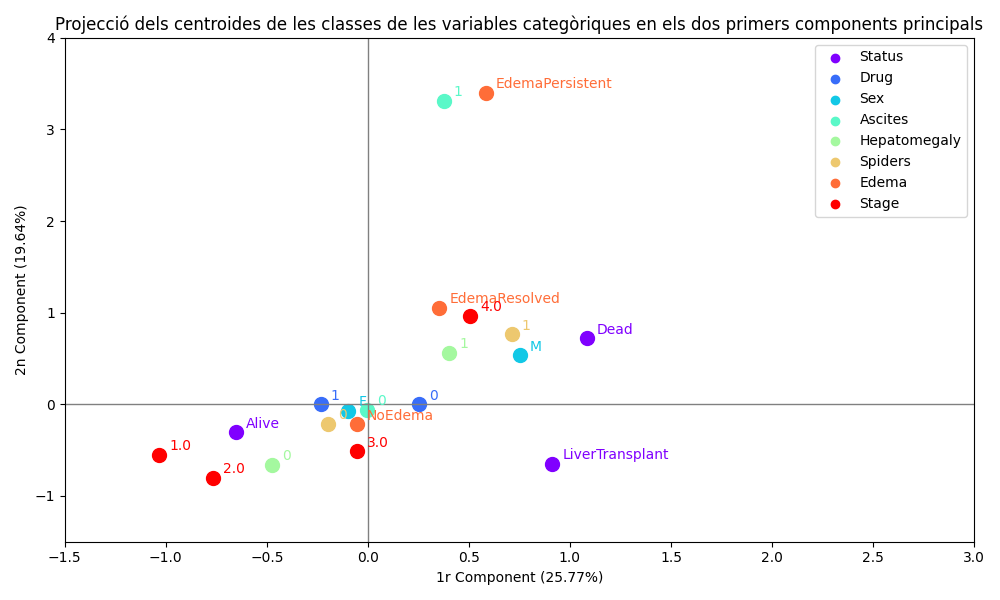
\includegraphics[width=0.9\textwidth]{img/acp_cat_vars_centroids.png}
    \caption{Projecció dels centroides de les classes de les variables categòriques en els dos primers components.}
    \label{fig:acp-cat-proj}
\end{figure}

Ajuntant la informació de les variables categòriques i de les numèriques (figures \ref{fig:acp-num-proj} i \ref{fig:acp-cat-proj}) podem dir que les variables numèriques que tenen més relació positiva amb la `Dead' són \textit{Copper} i \textit{Bilirubin}, mentre que \textit{Albumin} i \textit{N\_Days} tenen una relació positiva amb `Alive'. És a dir, tenen més probabilitats de sobreviure els pacients que tenen valors baixos de \textit{Copper} i \textit{Bilirubin} i valors alts de \textit{Albumin} i \textit{N\_Days}.

Com ja s'ha mencionat, aquestes conclusions no poden interpretar-se al peu de la lletra, ja que estan fetes sobre un 45\% de la variància explicada (i no pas un 100\%). No obstant, poden donar-nos unes nocions sobre les relacions entre variables, tant numèriques com categòriques com amb \textit{Status}.

En cas de que es desitgés fer una reducció de dimensionalitat per treballar amb components, les avantatges serien que hi hauria menys dimensions i seria més fàcil gestionar les dades. No obstant, s'ha de considerar que, com acabem de veure, es perd molta interpretabilitat i cada component passa a ser una barreja de conceptes i valors difícilment interpretable.

